\section{Layout}

The layout algorithm, determining the positions of sets and events within them,  consists of four steps. First, the vertical ordering of sets is computed to ensure that two sets that share events are next to each other wherever possible. Then, sets are further divided into layers, and events are assigned to them according to their memberships. After that, the position and length of each event are computed, within the given display space. Finally, layers are compacted to remove any gaps between them, before layer sizes are adjusted to allow for a consistent level of detail across all sets. 

\subsection{Sets Ordering}
\label{sec:set-ordering}
The set ordering algorithm aims to maximize the number of events shared by neighboring sets. This can be mapped to a graph path problem. Given a list of sets $S=\{s_1, s_2, \dotsc, s_n\}$, an undirected graph $G = (V,E)$ is created with each vertex $v_i$ represents a set $s_i \in S$. Two vertices $v_i$ and $v_j$ are connected if $s_i$ and $s_j$ share an event. The weight of edge $e_{ij}$ is the number of events shared by $s_i$ and $s_j$. Finding a set order with the maximum number of events shared by neighboring sets is equivalent to finding a path with the maximum weight connecting all vertices in $G$. This longest path problem is known to be NP-hard, but the number of sets we plan to support is limited by the number of colors that human can easily distinguish when they are shown together. Therefore, we decided on a brute-force approach to find the optimal solution.

\subsection{Layer Layout}
% Requirements
This algorithm positions all the events within a layer. Its inputs are:
\begin{itemize}
	\item The events belonging to the layer with their \emph{label} and \emph{time}.
	\item The maximum width and height of the layer.
\end{itemize}
The outputs are event locations within the constrained display area, optimizing for the following criteria:
\begin{description}
	\item[Completeness,] which measures how much event label is visible. More specifically, the \textit{completeness ratio} is defined as:
	$\theta = \frac{\alpha \cdot |E_c| + \beta \cdot |E_t|}{|E|}$
	, where $|E_c|$ is the number of complete events, $|E_t|$ is the number of trimmed events, and $|E|$ is the number of all events. $\alpha$ and $\beta$ are the coefficients to indicate how strongly a complete event and a trimmed event contributes to the overall content richness of the layer. We practically set $\alpha=1$ and $\beta=0.5$.
	
	\item[Traceability,]which measures how easy it is to follow the events chronologically. Events happened close in time should have small changes in their row levels to facilitate the tracing of them. More specifically, the \textit{traceability ratio} is defined as:
$	\gamma=\frac{\sum\limits_{i=1}^{|E|}(|l_{i+1} - l_i|)}{|E|-1}$
	, where $|E|$ is the number of all events within the layer and $l_i$ is the row level of event $e_i$. 	
\end{description}

The horizontal position of an event is fixed by its time. The layout algorithm decides on which row to position an event and the level of detail for its label.

\subsubsection{Completeness Algorithm}
Starting with an empty layer, the algorithm inserts events chronologically. An event is placed in the lowest possible row where it does not overlap with any other events. If such a row does not exist, one of the earlier events is trimmed to make space for it. Among these events, the one with the least trimming is selected. However, if the label space is too short for a single word after trimming, the event will be combined with the current event to form a new aggregated event titled ``2 events''. Aggregated events cannot be trimmed, thus a new event overlapping with them should also be aggregated. For example, a new event that overlaps with a ``2 events'' aggregated event will be aggregated, resulting in a ``3 events'' aggregated event. The completeness algorithm maximizes the number of complete events $|E_c|$ and trimmed events $|E_t|$, thus yielding a maximum completeness. This algorithm is not optimized for traceability because an event is placed in the lowest possible row disregarding the row level of its preceding event.

\subsubsection{Traceability Algorithm}
To improve traceability, this algorithm inserts a new event at the same row as its previous event. If there is an overlap, the previous event is trimmed to make space. The \emph{trim ratio} of an event is defined as the ratio of the remaining text length to its original length. An event can only be trimmed if the resulting trim ratio is greater than a minimum threshold $t_{min}$, where $0\leq t_{min} \leq 1$. This value determines how much completeness can be traded for traceability. If the resulting trim ratio is smaller than $t_{min}$, the event moves up or down to find a suitable row, up to $r_{max}$ rows on both sides. This value decides how far an event can be, in terms of row level difference, from the previous event, which essentially trades traceability for completeness. If no suitable row can be found within the +/- $r_{max}$ rows, the new event comes back to the level of its proceeding event, which is then trimmed or aggregated with the new event as in the completeness algorithm. Figure~\ref{fig:traceability} shows an example of these two algorithms used to layout seven events.

\begin{figure}[ht]
\centering
	\subcaptionbox{Completeness algorithm: $\theta=1$, $\gamma=5/3$.}{\label{fig:traceability1}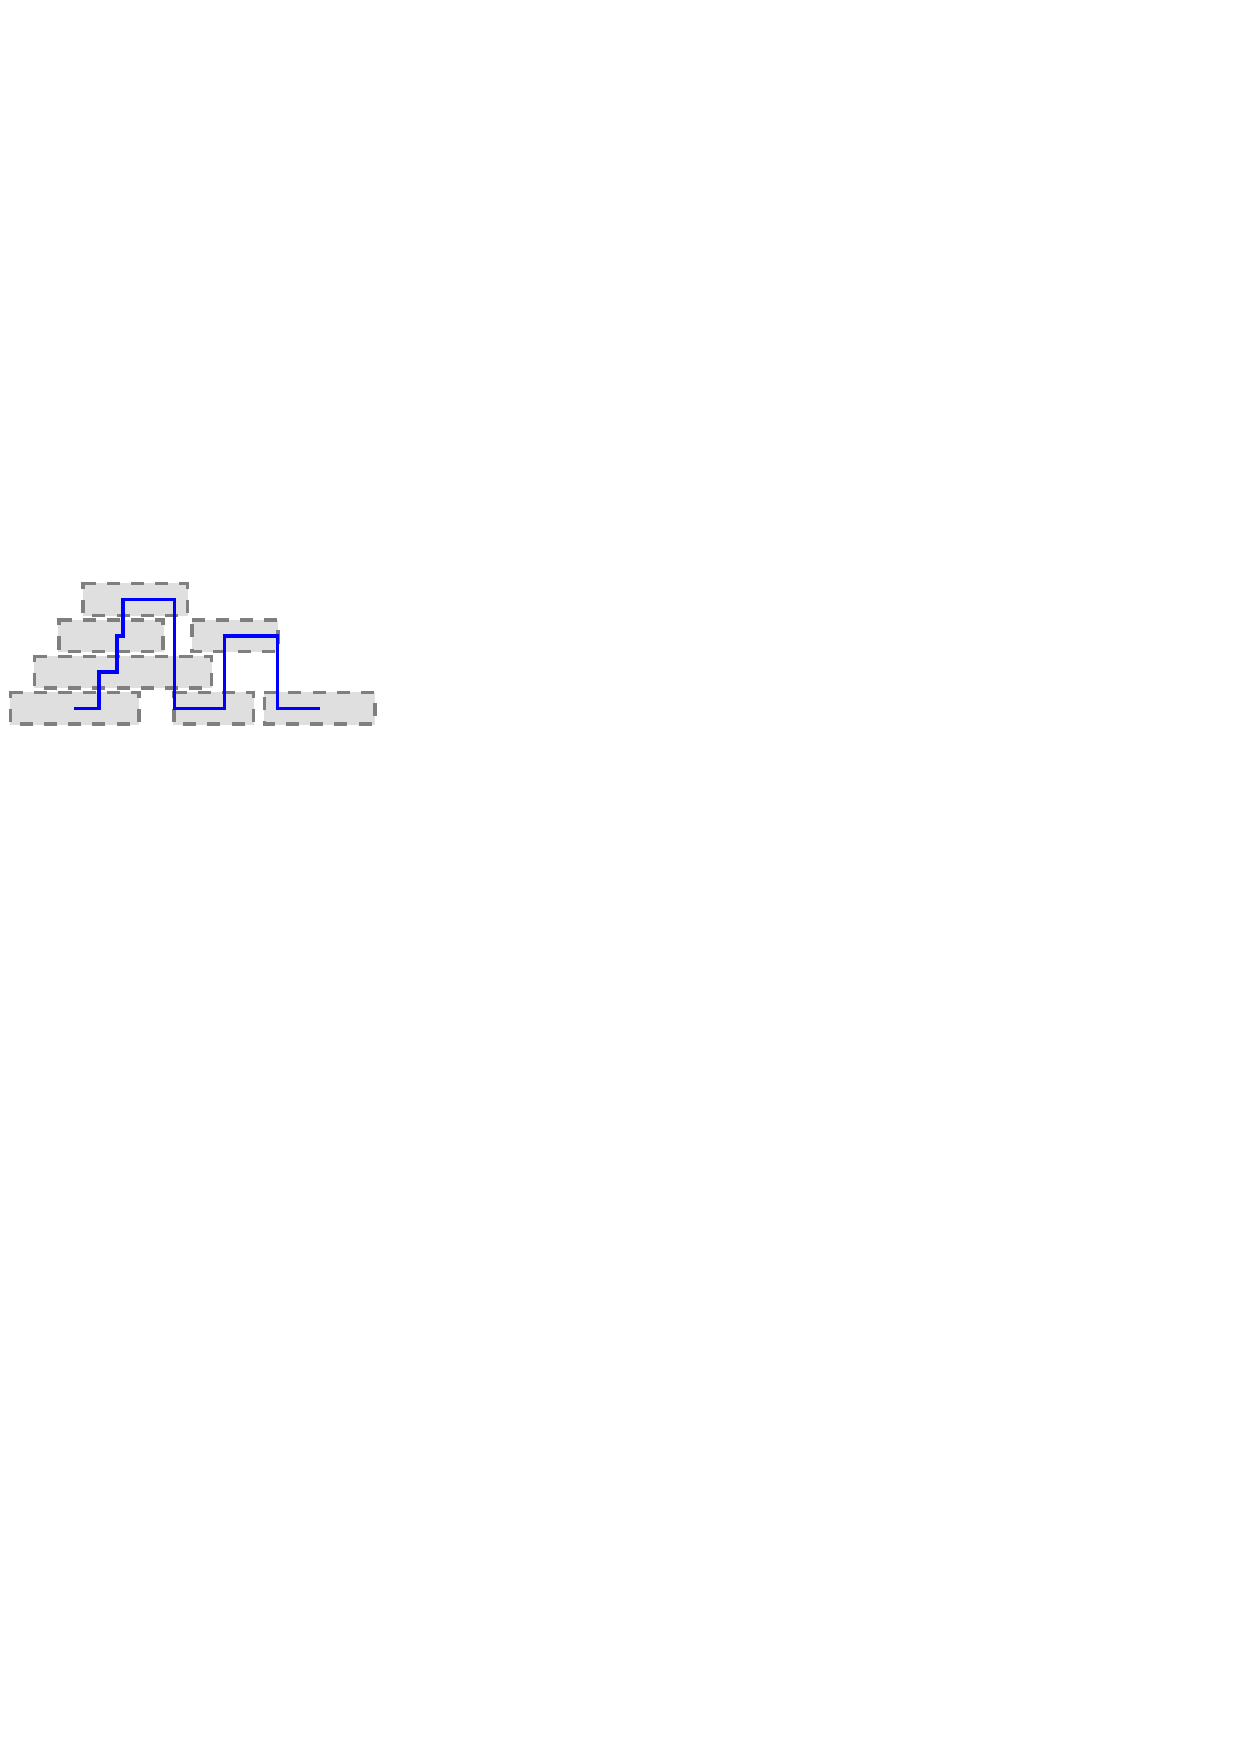
\includegraphics[width=.475\linewidth]{figure9a}}
	\hfill
	\subcaptionbox{Traceability algorithm ($t_{min}=0.5$, $r_{max}=1$): $\theta=6/7$, $\gamma=2/3$.}{\label{fig:traceability2}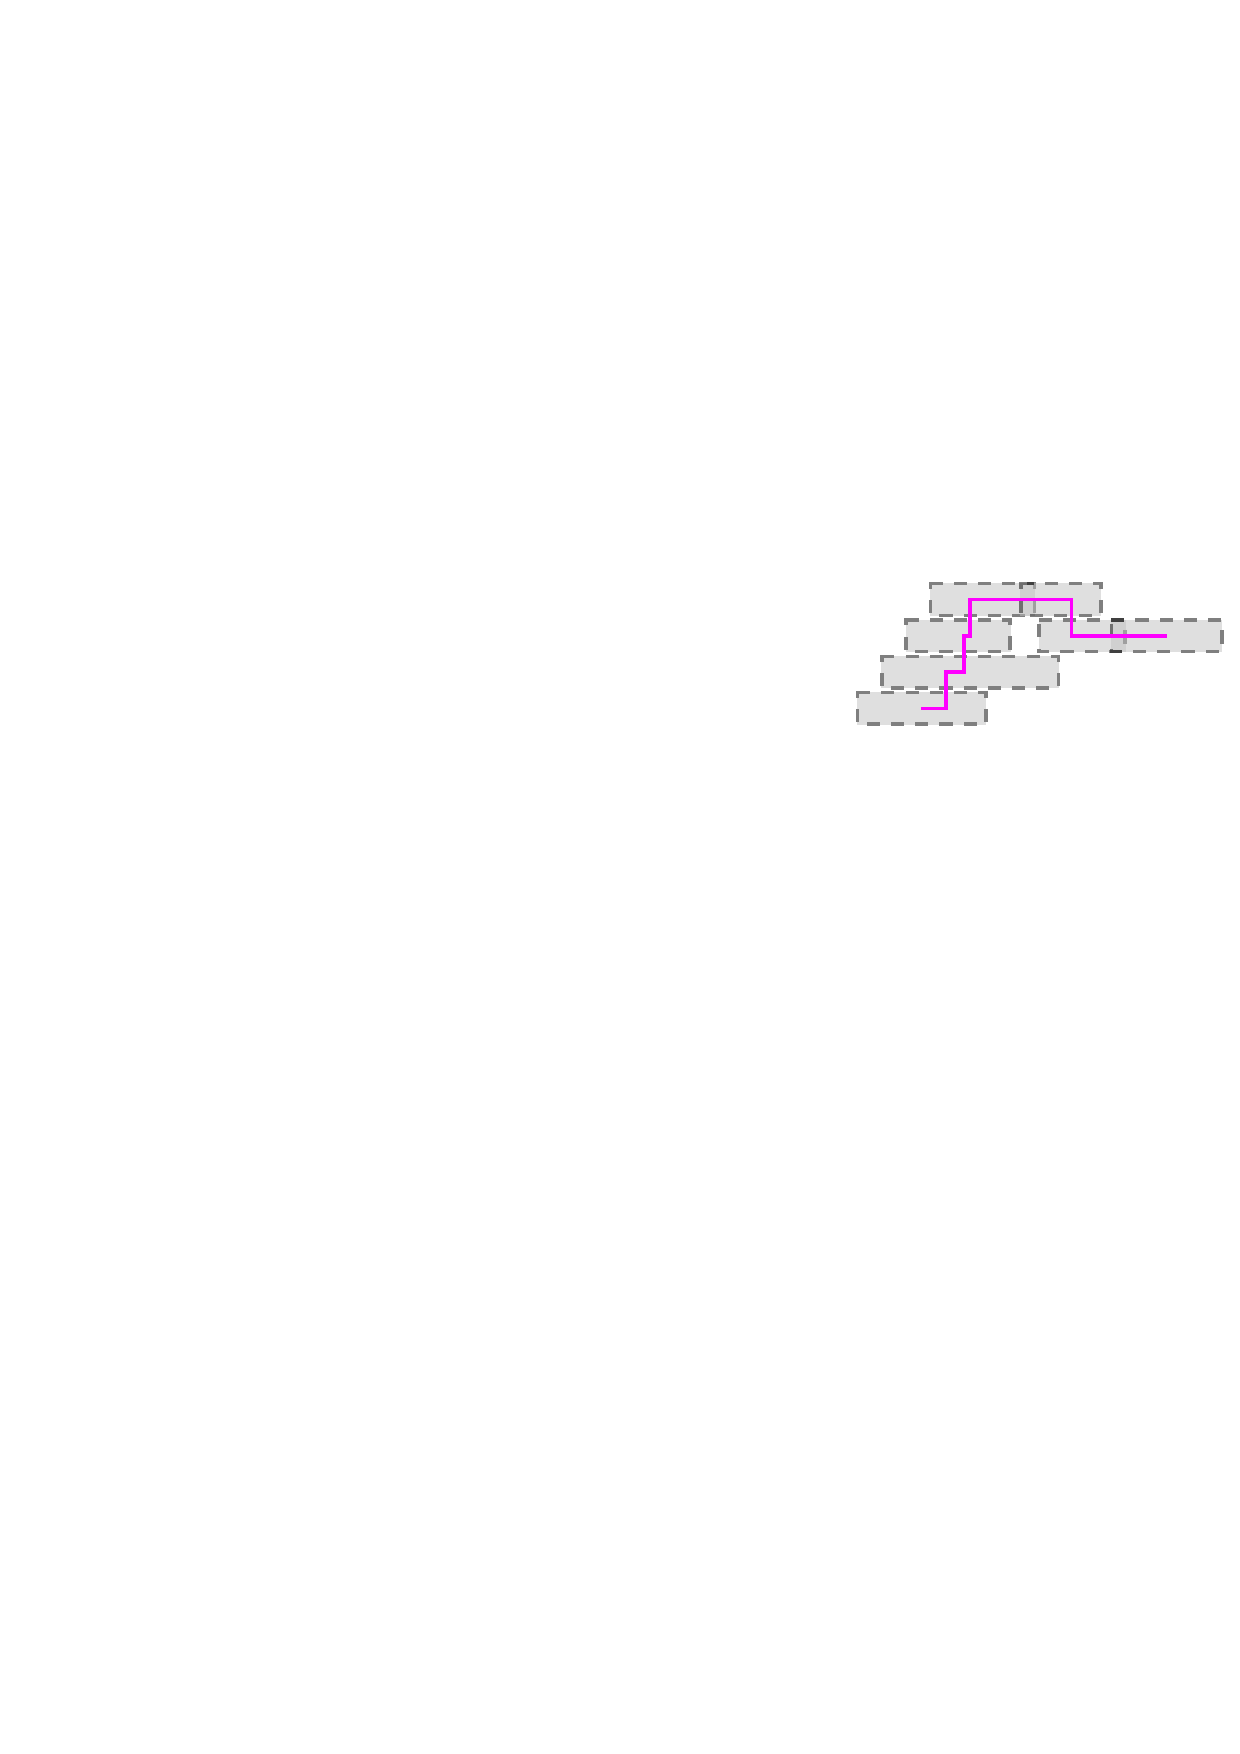
\includegraphics[width=.475\linewidth]{figure9b}}
\caption{Two layout algorithms. Each rectangle is the bounding box of an event with its label.}
\label{fig:traceability}
\end{figure}

Both layer layout algorithms run in linear time in terms of the number of events, because during the event insertion, the completeness algorithm checks up to a constant value -- the layer height, and the traceability algorithm checks at most ($2 \times r_{max}+1$) rows.

\subsection{Compacting}
\label{sub:compact}
The aforementioned layer layout needs a maximum number of rows it can use as an input. Initially, it is assigned proportionally to the number of events within each layer. After the layout of each layer is independently computed, some may be moved to fill the new space that appears between layers. This includes moving two layers closer if there is a gap in between, or moving a layer into a newly created space if its set does not share events with any other sets. Figure~\ref{fig:compacting} shows an example of compacting. The freed space is assigned to the layer with the lowest completeness ratio $\theta$. Then, layouts of all layers are recomputed and compacted again. The process repeats until no more space can be saved. 

\begin{figure}[ht]
	\centering
	\subcaptionbox{Before compacting.}{\label{fig:compacting1}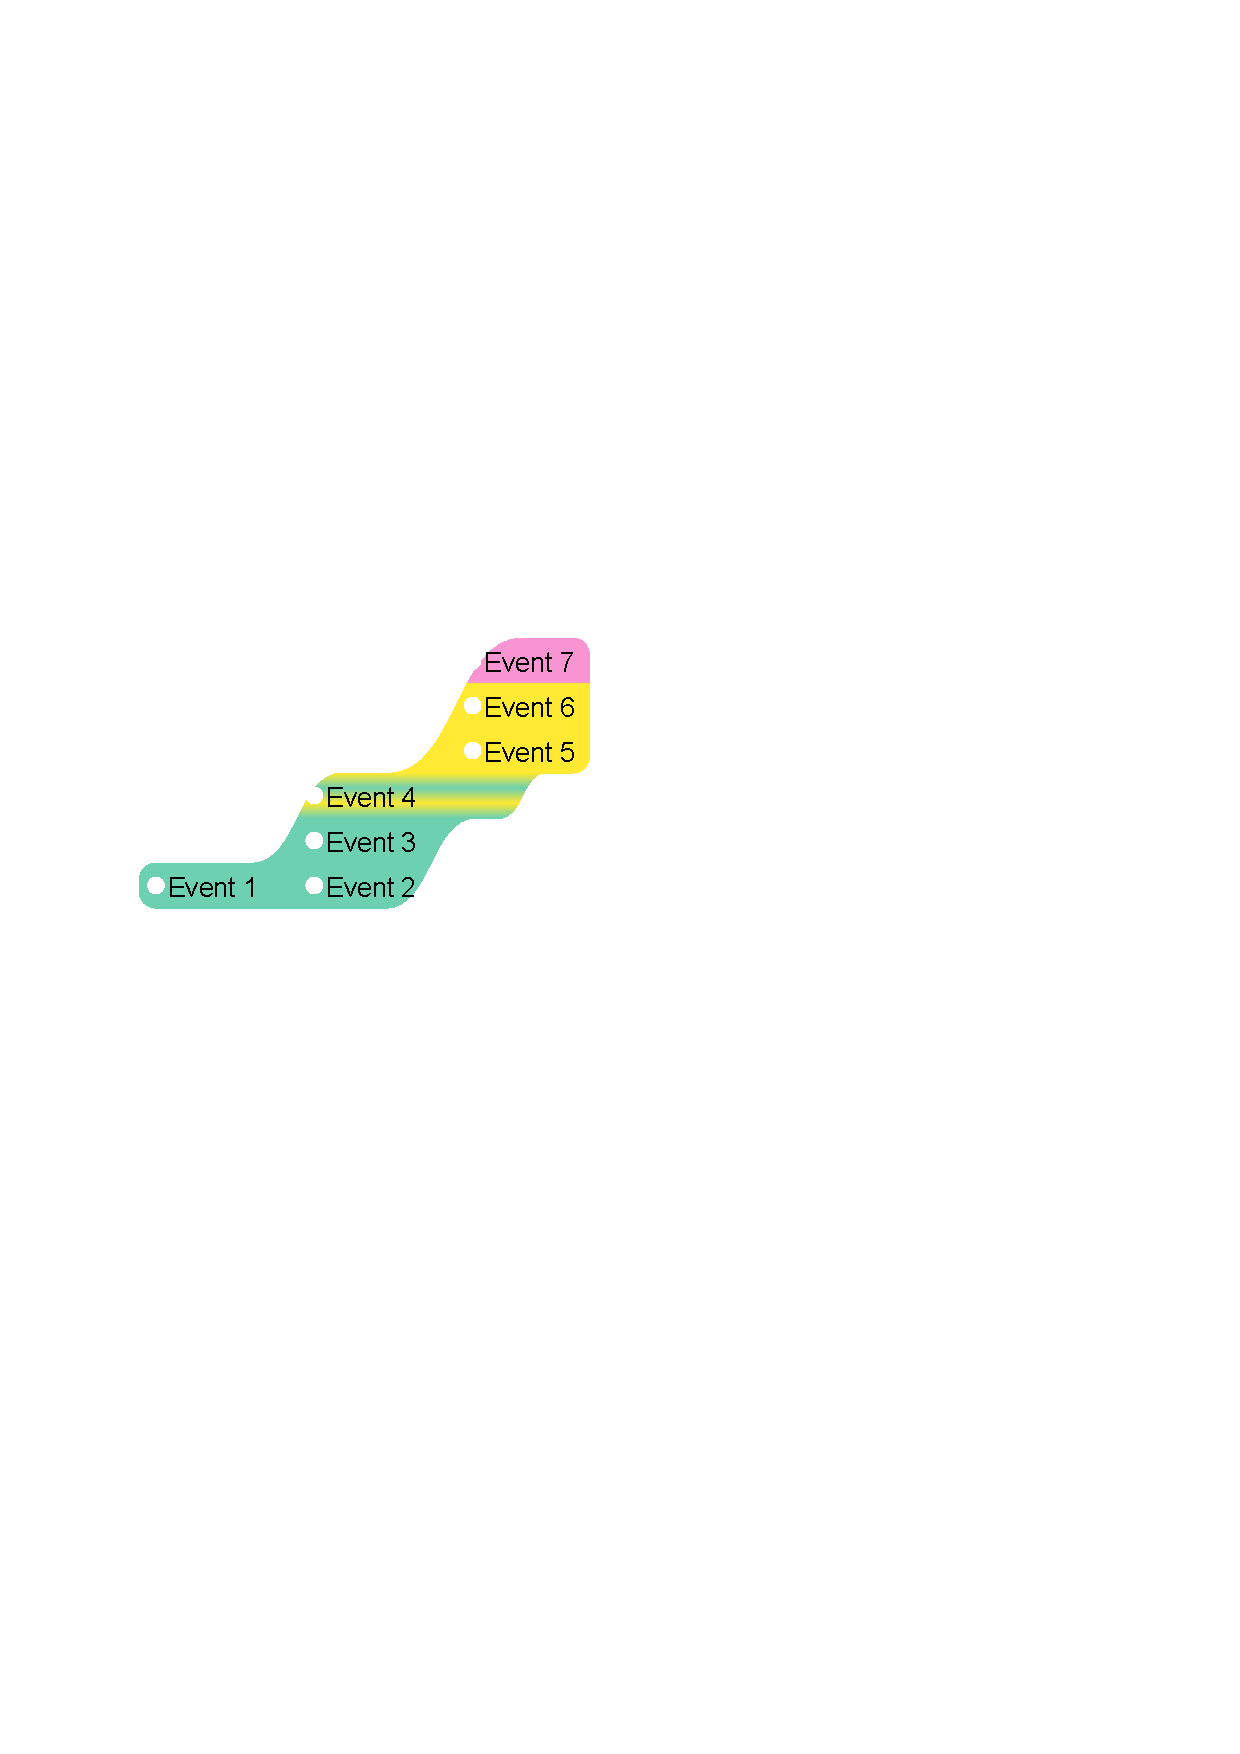
\includegraphics[width=.46\columnwidth]{figure10a}}
	\hfill
	\subcaptionbox{After compacting.}{\label{fig:compacting2}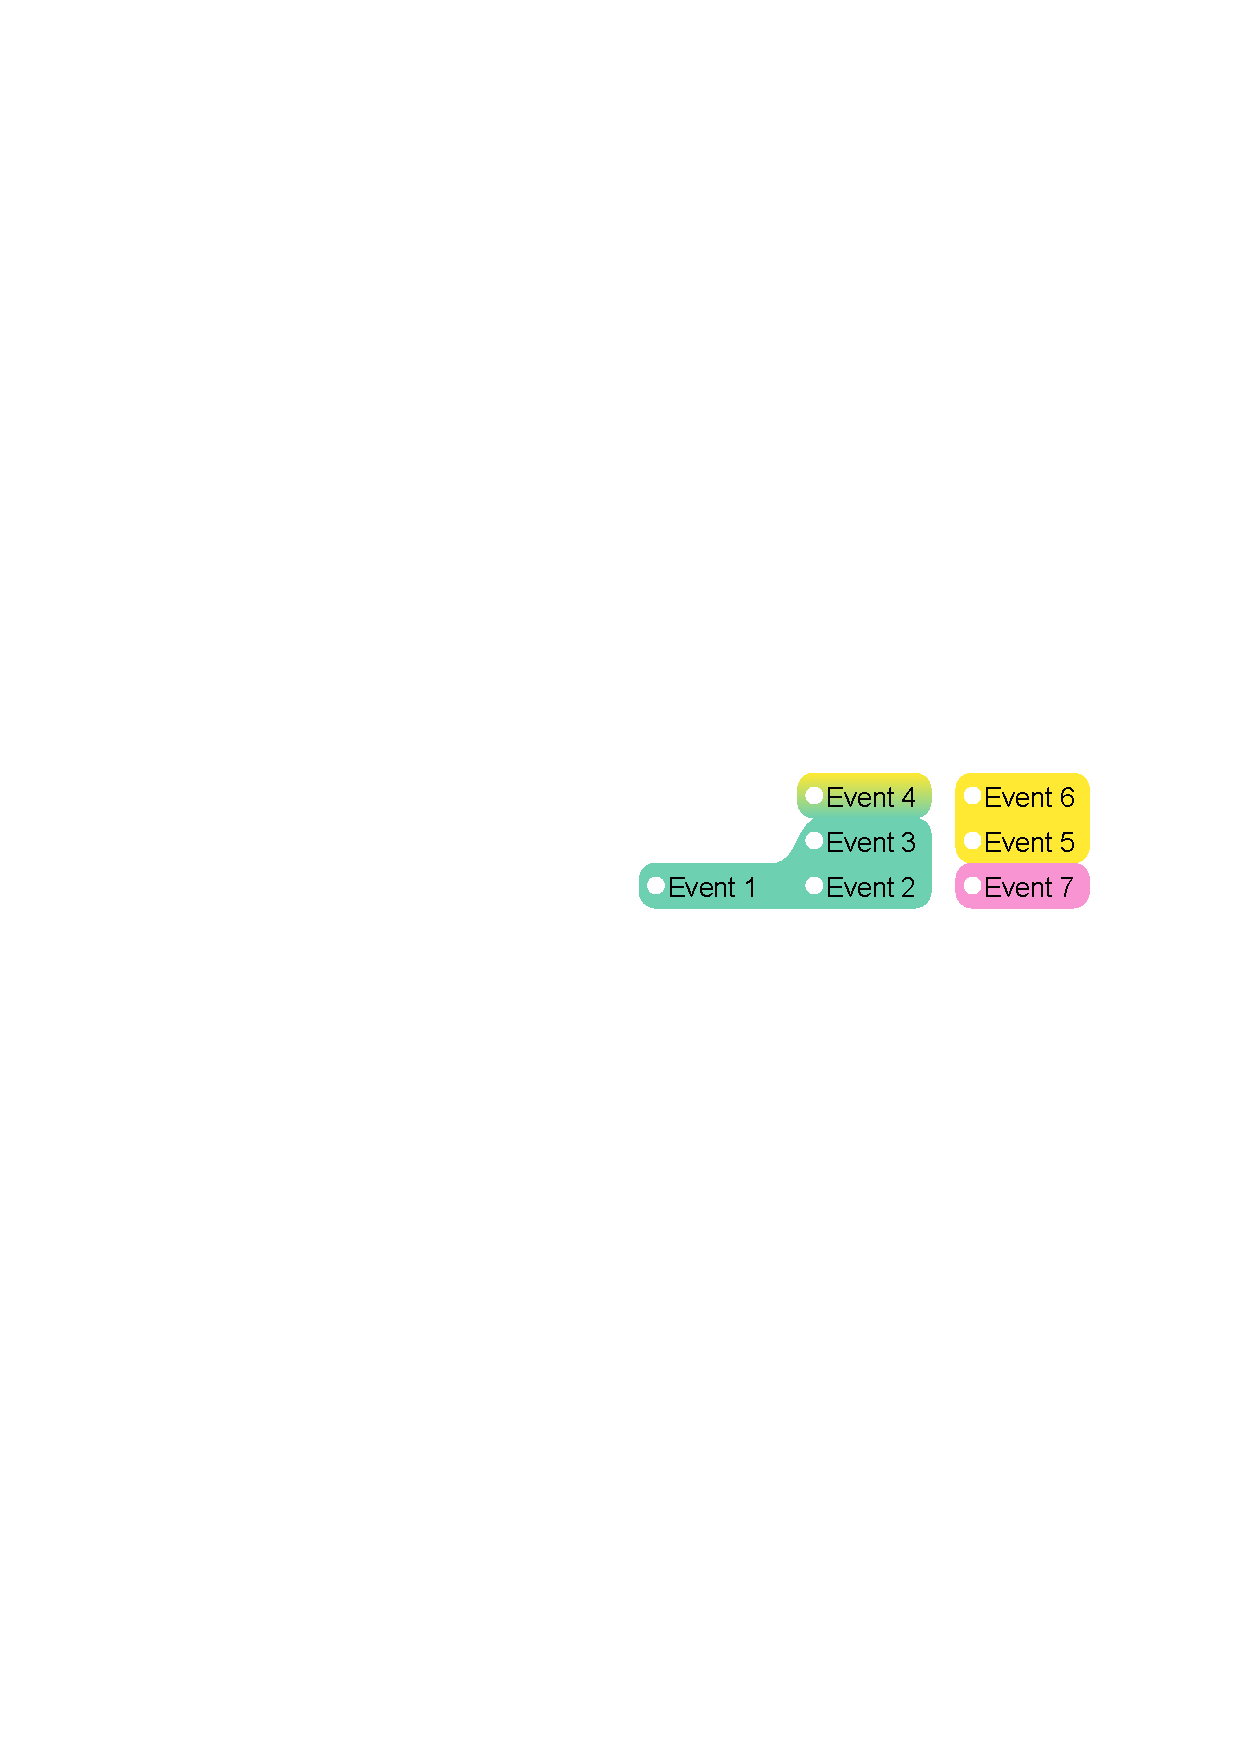
\includegraphics[width=.46\columnwidth]{figure10b}}
	\caption{Layer compacting example.}
	\label{fig:compacting}
\end{figure}

\subsection{Balancing}
This last step ensures that all the layers have similar levels of detail, i.e., it minimizes the variance of completeness,
$\frac{\sum\limits_{i=1}^{n}(\theta_i - \bar{\theta})^2} {n}$
, where $n$ is the number of layers and $\bar{\theta}$ is the mean of completeness ratio $\theta$. A brute force approach tests all possible combinations of layer height $h_i$ such that $\sum_{i=1}^{n}h_i=H$ for a minimum variance. However, the number of combinations is an exponential of $n$. Instead, we used a heuristic algorithm that relies on the fact that completeness ratio increases with layer height because there is more space to display labels. The algorithm reduces the completeness ratio variance by iteratively taking a row from the layer with the largest ratio and giving it to the layer with the smallest one, until the variance no longer decreases. Figure~\ref{fig:balancing} shows an example of balancing.

\begin{figure}[ht]
	\centering
	\subcaptionbox{Before balancing: $\theta_{green}=0.25$, $\theta_{yellow}=1$.}{\label{fig:balancing1}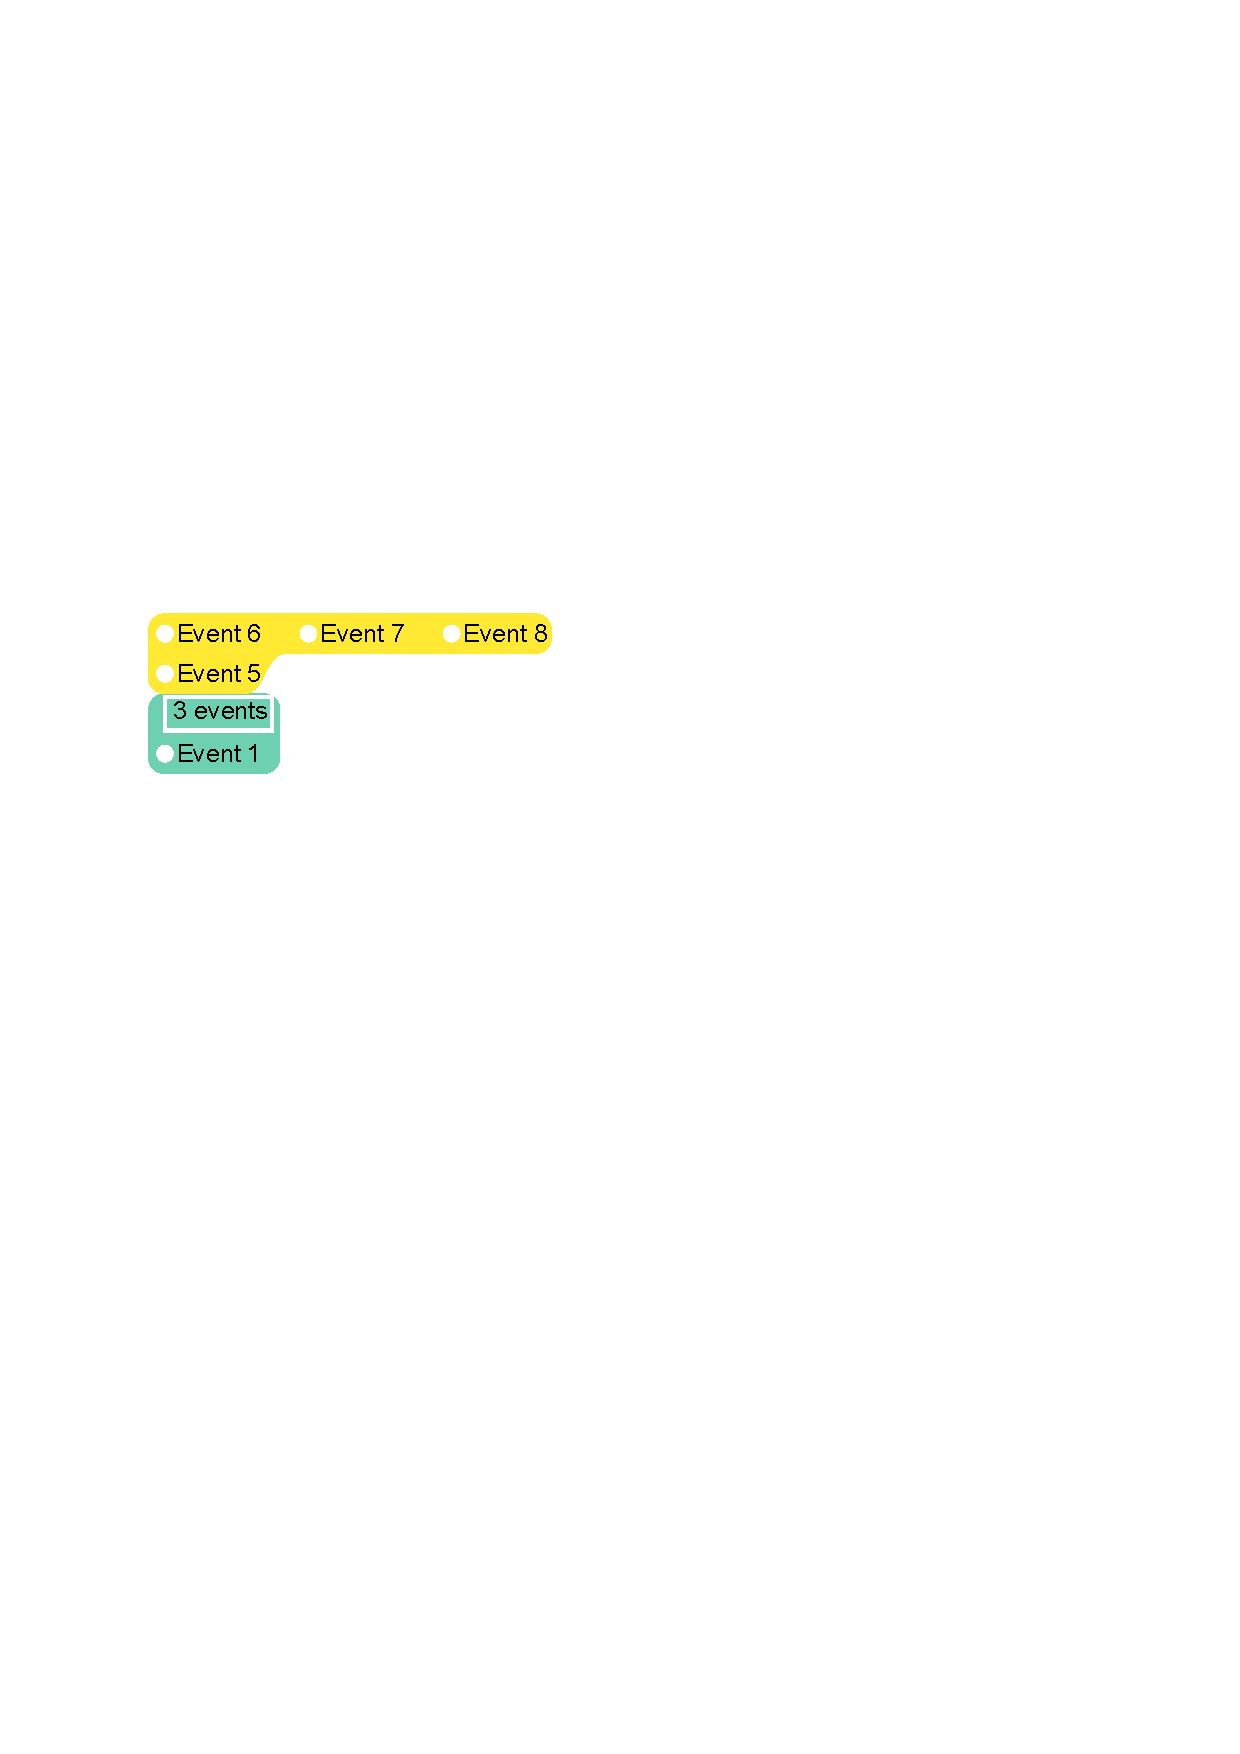
\includegraphics[width=.46\columnwidth]{figure11a}}
	\hfill
	\subcaptionbox{After balancing: $\theta_{green}=\theta_{yellow}=0.5$.}{\label{fig:balancing2}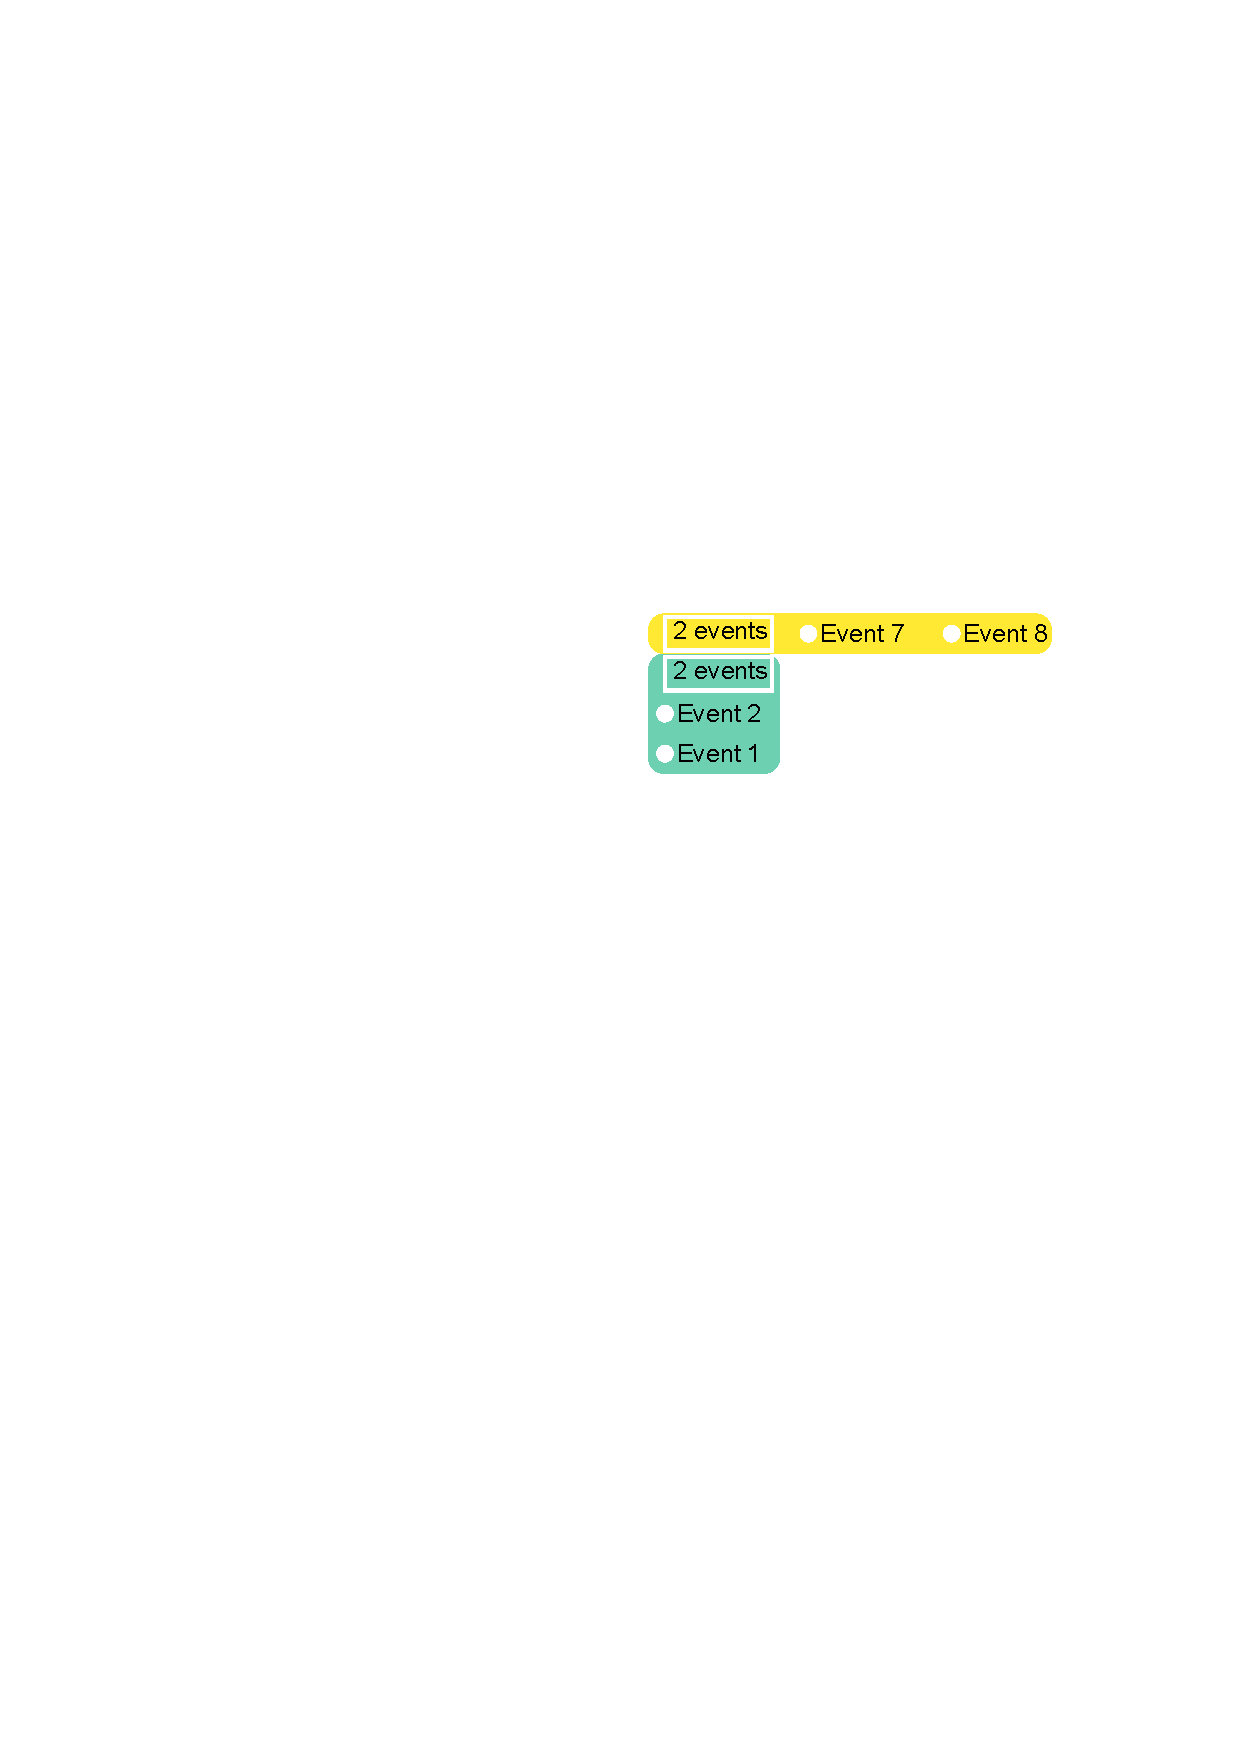
\includegraphics[width=.46\columnwidth]{figure11b}}
	\caption{Layer balancing example.}
	\label{fig:balancing}
\end{figure}

\subsection{Scalability}
Aggregation allows TimeSets to handle a large number of events. However, the visual encoding of aggregated events is imperfect: ``2 events'' and ``100 events'' are visually represented in the same way with rectangular border. Four options are considered to address this issue and illustrated in Figure~\ref{fig:aggreate}. First, the width of the bounding rectangle can be scaled to indicate the number of events (Figure~\ref{fig:aggregate-1}). However, the visual difference could be subtle and difficult to attract attention from an overview. The second option is to plot each individual event as a dot at when it happens (Figure~\ref{fig:aggregate-2}). This also provides a temporal distribution of events rather than just the quantity. When events happen at close or exactly the same time, dots are overlapped, and it is more difficult to see the pattern. Another approach is to color code the background of the bounding rectangle using luminance or intensity (Figure~\ref{fig:aggregate-3}). However, when many aggregated events are displayed, their backgrounds could interfere with the set colors. Last is to scale the font size of the label according to the number of events (Figure~\ref{fig:aggregate-4}). Currently, each event is completely placed in one single row with uniform height. Scaling the height of aggregated events needs to revise the layout algorithm.	All these methods have their strength and limitation, thus deciding the best one is challenging and out of scope for this paper. We leave the implementation and evaluation of these methods as future work.

\begin{figure}[ht]
	\centering
	\subcaptionbox{No encoding.}{\label{fig:aggregate-0}
		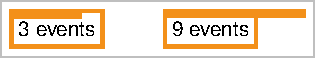
\includegraphics[width=.47\columnwidth]{figure12a}}
	\\
	\subcaptionbox{Scale with the width of the bounding rectangle.}{\label{fig:aggregate-1}
		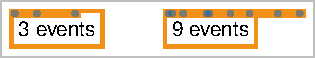
\includegraphics[width=.47\columnwidth]{figure12b}}
	\hfill
	\subcaptionbox{Each dot is an event at when it happens.}{\label{fig:aggregate-2}
		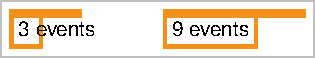
\includegraphics[width=.47\columnwidth]{figure12c}}
	\\
	\subcaptionbox{Color code the background of the bounding rectangle.}{\label{fig:aggregate-3}
		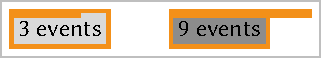
\includegraphics[width=.47\columnwidth]{figure12d}}
	\hfill
	\subcaptionbox{Scale with the font size of the label.}{\label{fig:aggregate-4}
		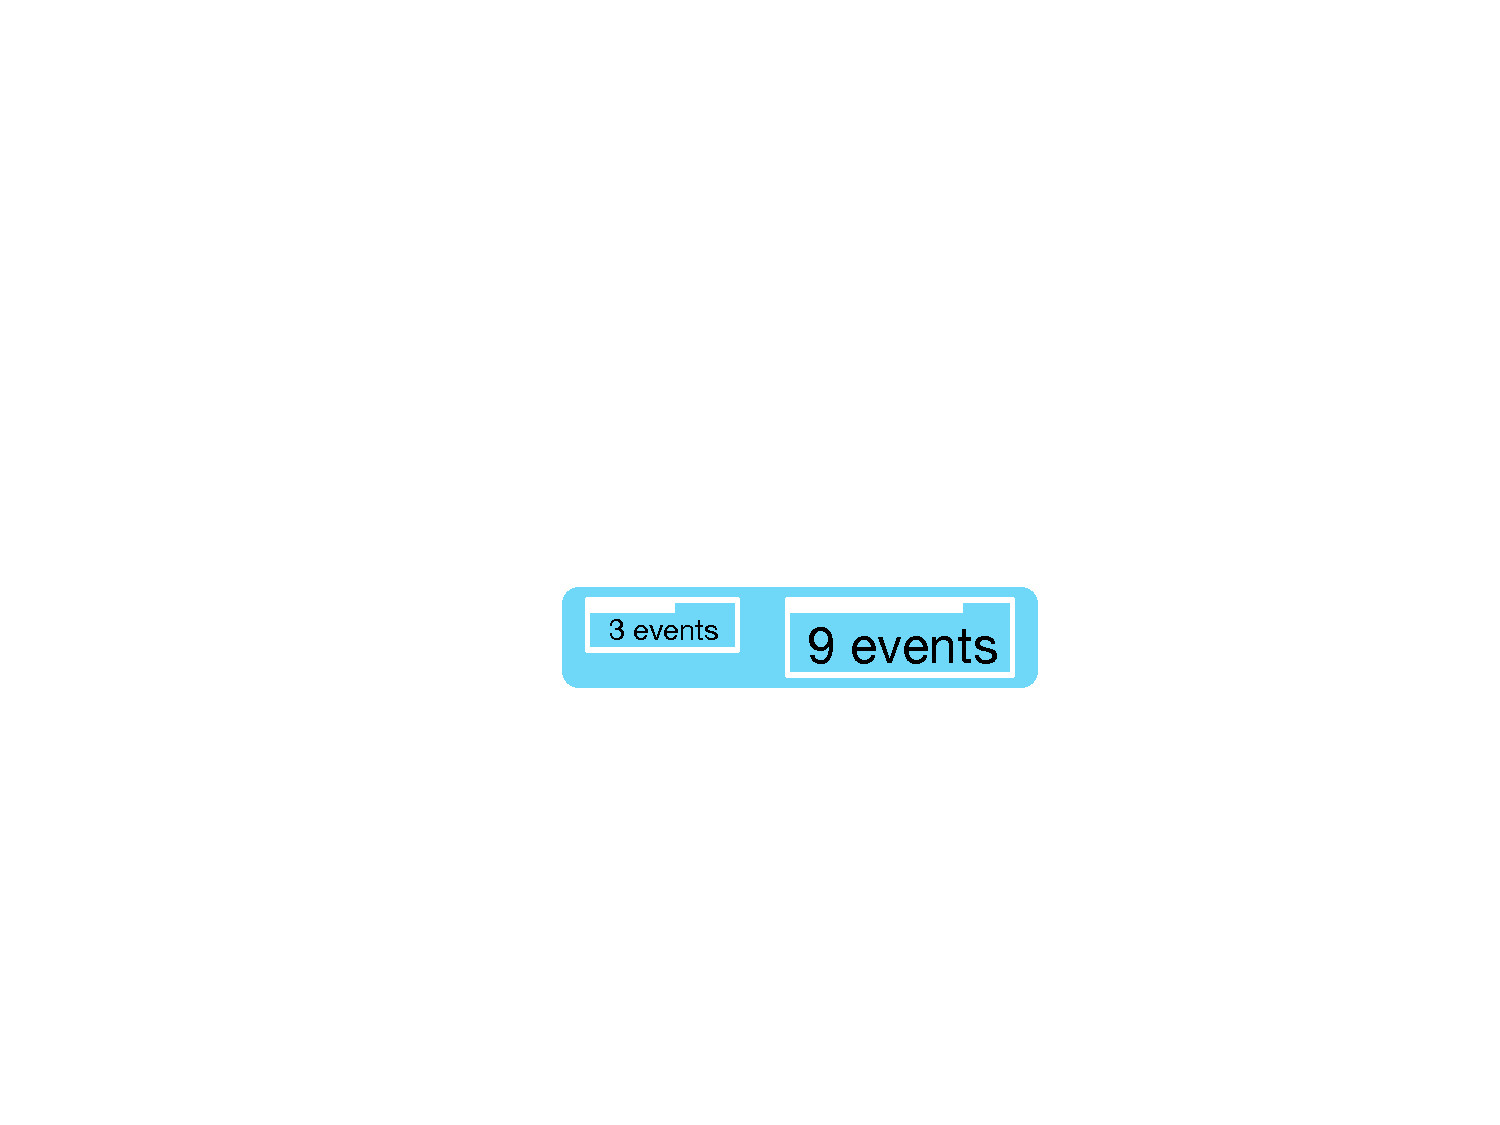
\includegraphics[width=.47\columnwidth]{figure12e}}
	\caption{Different visual representations of the number of events in an aggregate.}
	\label{fig:aggreate}
\end{figure}

The existing layout is suitable for a small timeline with a few hundreds of events or a detailed view where individual events are of high importance. Figure~\ref{fig:citations} shows 225 publications within 15 years. TimeSets relies on color to distinguish sets, therefore it is constrained by the number of colors that human can differentiate at the same time, which is about 12, according to Munzner's book~\cite{Munzner2014}.